%$$$$$$$$$$$$$$$$$$$$$$$$$$$$$$$$$$$$$$$$$$$$$$$$$$$$$$$$$$$$$$$$$$$$$$$$$$$$$$$$
%Paragraph 1:Linux Scalability의 연구에 대한 설명
%$$$$$$$$$$$$$$$$$$$$$$$$$$$$$$$$$$$$$$$$$$$$$$$$$$$$$$$$$$$$$$$$$$$$$$$$$$$$$$$$

\newpage
\section{최근 운영체제 병렬화 연구}
\label{sec:osrelated}

%To improve the scalability, researchers have attempted to create new
%operating systems~\cite{Boyd-WickizerCorey}~\cite{Wentzlaff2010fOS}
%~\cite{Baumann2009Barrelfish}~\cite{Zellweger2014Multikernel}
%~\cite{Liu2009Tessellation}~\cite{Farrington2010Helios}
%or have
% attempted to optimize existing operating
%
 % systems~\cite{SilasBoydWickizer2010LinuxScales48}~\cite{AustinTClements2012RCUBalancedTrees}~\cite{Clements2013RadixVM}~\cite{SilasBoydWickizerPth} ~\cite{Changwoo2016UMSF}.
 
코어 수가 증가되는 상황에서 병렬화가 중요해진 운영체제에 대한 연구는 성능에
 대한 확장성을 향상시키기 위해서, 새로운 확장성 있는
운영 체제를 만들거나 ~\cite{Boyd-WickizerCorey}~\cite{Wentzlaff2010fOS}
~\cite{Baumann2009Barrelfish}
~\cite{Liu2009Tessellation}~\cite{Farrington2010Helios} 
기존 운영체제를 최적화 시키는
방법~\cite{SilasBoydWickizer2010LinuxScales48}
~\cite{AustinTClements2012RCUBalancedTrees}~\cite{Clements2013RadixVM}~\cite{SilasBoydWickizerPth}을
시도하고 있다.

\subsection{새로운 운영체제 제안}

%Our research belongs to optimizing existing operating systems in order to
%solve the Linux fork scalability problem.
%이 중 우리의 연구는 리눅스의 fork에 대한 확장성을 개선하기 위한
% 기존 운영체제를 최적화 하는 방법에 속한다. 
%However, previous research did not deal with the anonymous reverse mapping,
%which is one of the fork scalability bottleneck.
%하지만 기존 연구들은 fork의 확장성 병목 지점 중 하나인 익명 역 매핑에 대해서는 처리하지 않았다.

%Cache-line fetches are expensive
%Read cache line written by
%another core: expensive!
%100–10000 cycles
%(contention)

%For reference, a creat system call costs 2.5K cycles
%Avoiding cache-line sharing is challenging
%Consider read-write lock
%struct readwritelock {
%int count;
%// -1, write mode; > 0, read mode
%listhead waiters;
%%spinlock waitlock;
%}
%Problem: to acquire lock in read mode requires modifying count
%%Fetching a remote cache line is expensive
%Many readers can cause performance collapse

\subsubsection{Corey}

Corey~\cite{Boyd-WickizerCorey}는 MIT의 Parallel and Distributed Operating Systems
Group에서 개발하였다.
기본적인 철학은 커널 영역의 공유 데이터를 유저 응용프로그램이 사용할 수 있게 만들어 주어서, 
공유 데이터 때문에 발생하는 경합 문제를 유저에게 해결할 수 있도록 공유에 대한 인터페이스를 제공하는 것이다. 
그 이유는 프로세서 내의 코어 간의 캐쉬 일관성 작업 때문에 성능이 저하되는데 이러한 것의 원인을 
운영체제가 응용프로그램과는 상관 없이 데이터를 공유하고 하드웨어 역시 응용프로그램에 상관없이 동기화 하는 
방식이기 때문에 기존의 운영체제에서 취하는 방법은 매니코어 환경에서 성능 향상이 어렵다는 것이다.  
따라서 유저 응용프로그램의 워크로드에 따라 공유 문제를 해결할 수 있는 방향을 제공해준다.
이것은 exokernel[]의 개념을 가져와서 매니코어 시스템에 적용하였고, 이를 통해 확장성을 개선하였다.

%$$$$$$$$$$$$$$$$$$$$$$$$$$$$$$$$$$$$$$$$$$$$$$$$$$$$$$$$$$$$$$$$$$$$$$$$$$$$$$$$
%Paragraph 2:Corey의 3가지 기본 개념 설명
%$$$$$$$$$$$$$$$$$$$$$$$$$$$$$$$$$$$$$$$$$$$$$$$$$$$$$$$$$$$$$$$$$$$$$$$$$$$$$$$$
이러한 Corey는 3가지 기본적은 개념을 가지고 있다. 그것은 공유(shares), 주소 트리(address trees)과 커널
코어(kernel core)이다.
공유는 어떻게 커널 자료구조를 접근할 수 있는지에 대해서 제공해준다.

\begin{figure}[h!]
    \centering
    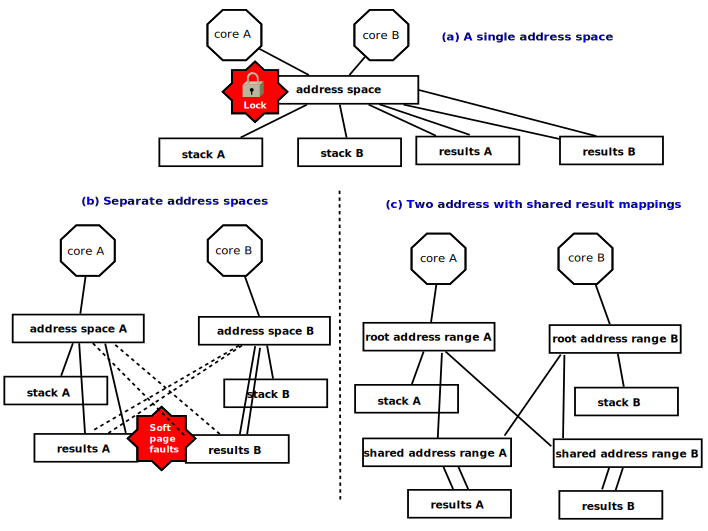
\includegraphics[width=1\textwidth]{fig/corey/corey}
    \caption{corey 운영체제 address space 공유 방법}
  \label{fig:corey}
\end{figure}

Non-blocking synchronization은 장점은 여러 스레드들이 락 기반으로 자원을 관리함에 따라
 발생하는 문제를 해결할 수 있다. 
가장 큰 장점은 스레드 또는 프로세스가 락 때문에 기다리는 시간을 제거할 수 있다.
이 것은 락을 얻기 위해 기다리는 시간을 최소화 할 뿐만 아니라 무한 루프 때문에 무한정 기다리는 
데드락 같은 상황까지 제거 할 수 있다. 
다음으로 모든 락은 락 자체의 오버헤드를 가지고 있는데 이것을 제거할 수 있다. 
예를 들어 코어 수가 증가 할 수록 락 자체를 얻기 위해 원자적 명령을 이용한느데 이것은 캐시 일관성 트래픽을 
발생한다. 
이와 같이 Non-blocking 방법은 이러한 락 자체가 가지고 있는 문제점인 데드락(deadlock), 라이브락(livelock), 
우선순위 역전현상(priority inversion)등을 제거 할 수 있다. 
이러한 Non-blocking synchronization 기법을 사용하는 lock-free 자료 구조들은 성능을 향상 시킬 수 있다. 
그 이유는 멀티코어 환경에서 공유되는 데이터를 접근하기 위해 직렬화 되는 부분이 매우 짧기 때문이다. 

\subsubsection{Barrelfish}

%$$$$$$$$$$$$$$$$$$$$$$$$$$$$$$$$$$$$$$$$$$$$$$$$$$$$$$$$$$$$$$$$$$$$$$$$$$$$$$$$
%Paragraph : Barrelfish의 특징 설명
%$$$$$$$$$$$$$$$$$$$$$$$$$$$$$$$$$$$$$$$$$$$$$$$$$$$$$$$$$$$$$$$$$$$$$$$$$$$$$$$$

Barrelfish~\cite{Baumann2009Barrelfish}는 취히리의 ETH와 마이크로 소프트(Microsoft)가
공동연구하여 만든 운영체제이다.
Barrelfish는 멀티커널(multikernel) 운영체제 중 하나이고, 
기본적인 철학은 공유 메모리 시스템 기능들을 모두 분산 처리 방식으로 구현하자는 것이다.
예를 들어, 운영체제에서 각 코어는 네트워크로 분산된 시스템으로 가정하고 메시지 패싱을 통해 분산된 
코어들간에 통신을 하여, 성능을 향상 시킨 방법이다. 
메시지 패싱 방법을 사용한 이유는, 오늘날 사용되는 캐시 구조로된 시스템의 
single shared interconnect가 코어가 증가할 수록 문제가 있기 때문에 하드웨어 cache coherence
protocol을 사용하는 방법보다 메시지 패싱 방법이 오히려 성능이 더 좋게 나오기 때문이다. 

%$$$$$$$$$$$$$$$$$$$$$$$$$$$$$$$$$$$$$$$$$$$$$$$$$$$$$$$$$$$$$$$$$$$$$$$$$$$$$$$$
%Paragraph : Barrelfish의 구조 설명 1
%$$$$$$$$$$$$$$$$$$$$$$$$$$$$$$$$$$$$$$$$$$$$$$$$$$$$$$$$$$$$$$$$$$$$$$$$$$$$$$$$

이러한 Barrelfish의 구조는 그림 x-x와 같이 하드웨어와 밀접한 CPU Driver와 이를 위해 Barrelfish 운영체제는
수직적인 측면에서 는 하드웨어에 밀접한 부분(CPU Driver)과 하드웨어 중립적인 부분(OS Node: (그림 8)에서 CPU
Driver위에 구현된 OS 서비스 모듈)으로 나누고, 운영체제 기능은 주로 OS Node에서 구현한다.
그리고 수평적 측면에서 는 다양한 하드웨어에 각각의 CPU Driver와 OS Node가 하나의 커널 역할을 하는 Multikernel
구조다. 그리고 이러한 커널은 메모리 공유 보다는 IPC를 통하여 통신을 하는 분산 구조이다.
 
\begin{figure}[h!]
    \centering
    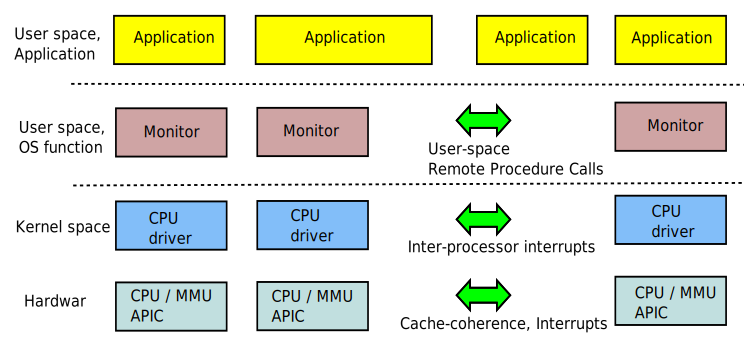
\includegraphics[width=1\textwidth]{fig/multikernel/multikernel}
    \caption{Barrelfish 구조}
  \label{fig:Barrelfish}
\end{figure}

%$$$$$$$$$$$$$$$$$$$$$$$$$$$$$$$$$$$$$$$$$$$$$$$$$$$$$$$$$$$$$$$$$$$$$$$$$$$$$$$$
%Paragraph : Barrelfish의 구조의 단점
%$$$$$$$$$$$$$$$$$$$$$$$$$$$$$$$$$$$$$$$$$$$$$$$$$$$$$$$$$$$$$$$$$$$$$$$$$$$$$$$$
Barrelfish의 구조적인 철학은 공유를 하지 말자는 것인데, 결국 이것은 로드 밸런싱을 수행할 수 
없는 구조로 되버린다. 예를 들어 하나의 코어에 많은 스레드들이 같이 돌고 있고, 다른 코어에는 아무런 
스레드도 없는 경우 분산 시스템 처럼 수행되므로, 동적으로 스레드에 대한 정보등을 다른 코어로 전송할 수가 없다.
즉 로드 밸런싱이 되지 않으므로 문제가 있다.

\subsubsection{fOS}


%$$$$$$$$$$$$$$$$$$$$$$$$$$$$$$$$$$$$$$$$$$$$$$$$$$$$$$$$$$$$$$$$$$$$$$$$$$$$$$$$
%Paragraph : fOS의 특징 설명
%$$$$$$$$$$$$$$$$$$$$$$$$$$$$$$$$$$$$$$$$$$$$$$$$$$$$$$$$$$$$$$$$$$$$$$$$$$$$$$$$

fOS(Factored operating system)~\cite{Wentzlaff2010fOS}은 역시 Massachusetts
Instiute of Technoloy에서 개발한 Corey와 비슷한 개념의 운영체제이다.
fOS의 5가지의 설계 철학을 가지고 있다. 

Non-blocking synchronization은 장점은 여러 스레드들이 락 기반으로 자원을 관리함에 따라
 발생하는 문제를 해결할 수 있다. 
가장 큰 장점은 스레드 또는 프로세스가 락 때문에 기다리는 시간을 제거할 수 있다.
이 것은 락을 얻기 위해 기다리는 시간을 최소화 할 뿐만 아니라 무한 루프 때문에 무한정 기다리는 
데드락 같은 상황까지 제거 할 수 있다. 
다음으로 모든 락은 락 자체의 오버헤드를 가지고 있는데 이것을 제거할 수 있다. 
예를 들어 코어 수가 증가 할 수록 락 자체를 얻기 위해 원자적 명령을 이용한느데 이것은 캐시 일관성 트래픽을 
발생한다. 
이와 같이 Non-blocking 방법은 이러한 락 자체가 가지고 있는 문제점인 데드락(deadlock), 라이브락(livelock), 
우선순위 역전현상(priority inversion)등을 제거 할 수 있다. 
이러한 Non-blocking synchronization 기법을 사용하는 lock-free 자료 구조들은 성능을 향상 시킬 수 있다. 
그 이유는 멀티코어 환경에서 공유되는 데이터를 접근하기 위해 직렬화 되는 부분이 매우 짧기 때문이다. 

%$$$$$$$$$$$$$$$$$$$$$$$$$$$$$$$$$$$$$$$$$$$$$$$$$$$$$$$$$$$$$$$$$$$$$$$$$$$$$$$$
%Paragraph : fOS의 구조 설명
%$$$$$$$$$$$$$$$$$$$$$$$$$$$$$$$$$$$$$$$$$$$$$$$$$$$$$$$$$$$$$$$$$$$$$$$$$$$$$$$$
Non-blocking synchronization은 장점은 여러 스레드들이 락 기반으로 자원을 관리함에 따라
 발생하는 문제를 해결할 수 있다. 
가장 큰 장점은 스레드 또는 프로세스가 락 때문에 기다리는 시간을 제거할 수 있다.
이 것은 락을 얻기 위해 기다리는 시간을 최소화 할 뿐만 아니라 무한 루프 때문에 무한정 기다리는 
데드락 같은 상황까지 제거 할 수 있다. 
다음으로 모든 락은 락 자체의 오버헤드를 가지고 있는데 이것을 제거할 수 있다. 
예를 들어 코어 수가 증가 할 수록 락 자체를 얻기 위해 원자적 명령을 이용한느데 이것은 캐시 일관성 트래픽을 
발생한다. 
이와 같이 Non-blocking 방법은 이러한 락 자체가 가지고 있는 문제점인 데드락(deadlock), 라이브락(livelock), 
우선순위 역전현상(priority inversion)등을 제거 할 수 있다. 
이러한 Non-blocking synchronization 기법을 사용하는 lock-free 자료 구조들은 성능을 향상 시킬 수 있다. 
그 이유는 멀티코어 환경에서 공유되는 데이터를 접근하기 위해 직렬화 되는 부분이 매우 짧기 때문이다. 


\subsubsection{Fused OS}

%$$$$$$$$$$$$$$$$$$$$$$$$$$$$$$$$$$$$$$$$$$$$$$$$$$$$$$$$$$$$$$$$$$$$$$$$$$$$$$$$
%Paragraph : Fused OS의 특징 설명
%$$$$$$$$$$$$$$$$$$$$$$$$$$$$$$$$$$$$$$$$$$$$$$$$$$$$$$$$$$$$$$$$$$$$$$$$$$$$$$$$
Fused OS는 IBM 연구소에서 개발되었으며, 모노리틱 구조와 마이크로 구조의 장점을 혼합한 구조이다. 
이것이 기본철학은 시간과 공간을 파티션하여 동작시키도록 만든 하나의 파티션닝 운영체제이다.

IBM 왓슨 연구소에서 모노리틱 구조의 운영체제와
마이크로 커널 구조의 운영체제의 장점을 혼합한 구조
의 운영체제(Fused OS)를 연구[12][13]하였다. IBM
Blue Gene/Q 시스템에서 HPC 응용을 성능 확장성이
있고 신뢰성 있게 수행시키는 것이 주목적이지만, 이질
적인(heterogeneous) 코어로 구성된 Manycore 시스템
의 운영체제 구조 연구가 시작점이었다. 여기서 이질적
인 코어란 전력 효율적인 코어(PEC: Power Efficient
Core)와 단일 쓰레드에 성능 최적화된 코어(STOC:
Single Thread Optimized Core)로 구성된 프로세스 코
어 칩을 의미한다. 따라서 Fused OS 설계개념은 응용과
운영체제를 다른 코어에서 수행되도록 하여 응용의 성
능이 운영체제에 의해 간섭을 받지 않도록 하는 것이다.

\begin{figure}[h!]
    \centering
    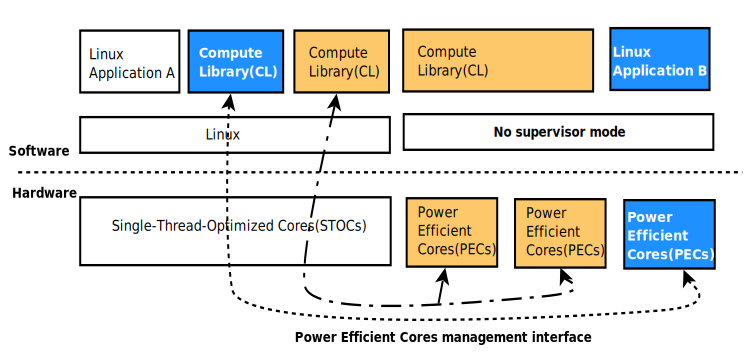
\includegraphics[width=1\textwidth]{fig/fusedos/fusedos}
    \caption{FusedOS 구조}
  \label{fig:FusedOS}
\end{figure}

%$$$$$$$$$$$$$$$$$$$$$$$$$$$$$$$$$$$$$$$$$$$$$$$$$$$$$$$$$$$$$$$$$$$$$$$$$$$$$$$$
%Paragraph : Fused OS의 구조 설명
%$$$$$$$$$$$$$$$$$$$$$$$$$$$$$$$$$$$$$$$$$$$$$$$$$$$$$$$$$$$$$$$$$$$$$$$$$$$$$$$$
같이 Fused OS의 기본 동작은 응용과 운
영체제가 다른 코어에서 각각 수행되는 것이다.
를 저장하고 리눅스 운영체제에게 전달하는 역할을 한
다. 반면에 리눅스 운영체제는 기존의 리눅스 코드에
PEC 코어의 메모리 등을 접근할 수 있는 기능을 추가하
였다. 게다가 PEC 코어를 관리하는 CL(Compute
Library)이 리눅스 응용으로 동작하며, 이 CL은 가벼운
커널 기능을 가지고 있게 설계되었다. 즉 리눅스 운영체
제에서 만들어진 응용이 PEC 코어에서 수행되기 위해
서, CL는 PEC 메모리에 응용 이미지를 구축하고 수행
되도록 PEC 코어에 전달하게 된다. 따라서 Fused OS는
코어와 메모리 자원을 분할하여, HPC 응용의 성능을 보
장하면서 리눅스 운영체제 기능도 제공하게 되었다.
HPC 벤치마킹 결과, Fused OS는 운영체제 기능을
하는 코어와 계산을 위한 코어를 분리시켰기 때문에, 성
능 측면에서 계산을 위한 코어에서 실행되는 응용은 운
영체제 기능을 하는 코어에서 실행하는 응용보다 우수
하다는 것을 밝혔다. 하지만 응용에서 호출하는 시스템
호출은 원격의 운영체제 코어에서 처리되기 때문에 추
가적인 호출시간이 필요하다.


\subsection{기존 운영체제 최적화}

\subsubsection{Linux scalability}

MIT PDOS 연구 그룹은 새로운 운영체제가 아닌 리눅스 커널을 대상으로 매니코어 환경에서 확장성을 연구하였다.
실제 사용되는 7가지의 응용프로그램을 가지고 MOSBENCH라는 응용프로그램 벤치마크를 만들어 리눅스 커널을 대상으로 
성능을 측정하였고, 그 도중 발생되는 여러 문제를 해결하여, 성능을 향상시켰다.

\begin{figure}[h!]
    \centering
    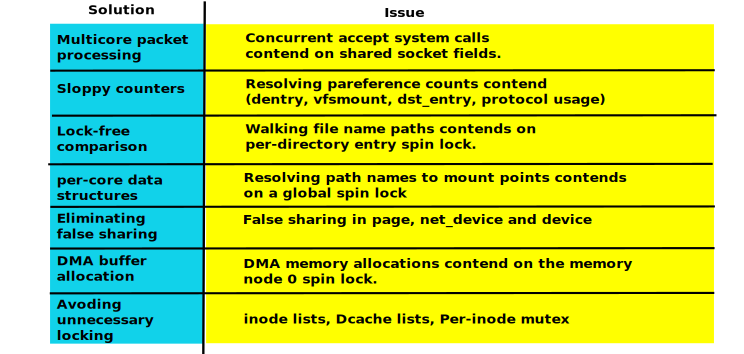
\includegraphics[width=1\textwidth]{fig/linux/linux}
    \caption{linux scalability 분석 연구}
  \label{fig:linux}
\end{figure}


표 x-x와 같이 총 9가지의 기술을 활용과 응용프로그램을 직접 수정하여 커널 확장성을 개선하였다.
%$$$$$$$$$$$$$$$$$$$$$$$$$$$$$$$$$$$$$$$$$$$$$$$$$$$$$$$$$$$$$$$$$$$$$$$$$$$$$$$$
%Paragraph : 9가지의 기술에 대한 설명 1
%$$$$$$$$$$$$$$$$$$$$$$$$$$$$$$$$$$$$$$$$$$$$$$$$$$$$$$$$$$$$$$$$$$$$$$$$$$$$$$$$
Non-blocking synchronization은 장점은 여러 스레드들이 락 기반으로 자원을 관리함에 따라
 발생하는 문제를 해결할 수 있다. 
가장 큰 장점은 스레드 또는 프로세스가 락 때문에 기다리는 시간을 제거할 수 있다.
이 것은 락을 얻기 위해 기다리는 시간을 최소화 할 뿐만 아니라 무한 루프 때문에 무한정 기다리는 
데드락 같은 상황까지 제거 할 수 있다. 
다음으로 모든 락은 락 자체의 오버헤드를 가지고 있는데 이것을 제거할 수 있다. 
예를 들어 코어 수가 증가 할 수록 락 자체를 얻기 위해 원자적 명령을 이용한느데 이것은 캐시 일관성 트래픽을 
발생한다. 
이와 같이 Non-blocking 방법은 이러한 락 자체가 가지고 있는 문제점인 데드락(deadlock), 라이브락(livelock), 
우선순위 역전현상(priority inversion)등을 제거 할 수 있다. 
이러한 Non-blocking synchronization 기법을 사용하는 lock-free 자료 구조들은 성능을 향상 시킬 수 있다. 
그 이유는 멀티코어 환경에서 공유되는 데이터를 접근하기 위해 직렬화 되는 부분이 매우 짧기 때문이다. 

%$$$$$$$$$$$$$$$$$$$$$$$$$$$$$$$$$$$$$$$$$$$$$$$$$$$$$$$$$$$$$$$$$$$$$$$$$$$$$$$$
%Paragraph : 9가지의 기술에 대한 설명 2
%$$$$$$$$$$$$$$$$$$$$$$$$$$$$$$$$$$$$$$$$$$$$$$$$$$$$$$$$$$$$$$$$$$$$$$$$$$$$$$$$

Non-blocking synchronization은 장점은 여러 스레드들이 락 기반으로 자원을 관리함에 따라
 발생하는 문제를 해결할 수 있다. 
가장 큰 장점은 스레드 또는 프로세스가 락 때문에 기다리는 시간을 제거할 수 있다.
이 것은 락을 얻기 위해 기다리는 시간을 최소화 할 뿐만 아니라 무한 루프 때문에 무한정 기다리는 
데드락 같은 상황까지 제거 할 수 있다. 
다음으로 모든 락은 락 자체의 오버헤드를 가지고 있는데 이것을 제거할 수 있다. 
예를 들어 코어 수가 증가 할 수록 락 자체를 얻기 위해 원자적 명령을 이용한느데 이것은 캐시 일관성 트래픽을 
발생한다. 
이와 같이 Non-blocking 방법은 이러한 락 자체가 가지고 있는 문제점인 데드락(deadlock), 라이브락(livelock), 
우선순위 역전현상(priority inversion)등을 제거 할 수 있다. 
이러한 Non-blocking synchronization 기법을 사용하는 lock-free 자료 구조들은 성능을 향상 시킬 수 있다. 
그 이유는 멀티코어 환경에서 공유되는 데이터를 접근하기 위해 직렬화 되는 부분이 매우 짧기 때문이다. 

\subsubsection{BonsaiVM}

%$$$$$$$$$$$$$$$$$$$$$$$$$$$$$$$$$$$$$$$$$$$$$$$$$$$$$$$$$$$$$$$$$$$$$$$$$$$$$$$$
%Paragraph : BonsaiVM 특징 설명
%$$$$$$$$$$$$$$$$$$$$$$$$$$$$$$$$$$$$$$$$$$$$$$$$$$$$$$$$$$$$$$$$$$$$$$$$$$$$$$$$
BonsaiVM은 MIT Parallel and Distributed Operating Systems Group에서 개발한 리눅스 커널을 위한 
가상 메모리 시스템이다. 
리눅스의 멀티 스레드들은 하나의 address space를 공유하게 되는데, 이러한 공유된 address space 때문에 
mmap과 soft page fault간에 공유된 address space를 보호하기 위해, reader-writer 세마포어를 사용한다. 
하지만, 많은 경합 때문에 스레들이 블락 걸리는 현상이 많이 생기는데 이 때문에 코어가 많아 지면 성능이 떨어지는 
문제가 있다. 
이러한 single address space 문제해결하기 위해서 앞에서 설명한 corey 운영체제를 만드는 등 여러 연구들이 
진행되었지만, 이 연구에서는 여러 기법을 적용한 새로운 VM과 RCU라는 리눅스 커널의 동기화 기법을 사용하여 
이 문제를 해결하였다. 
이것은 새로운 운영체제를 제안하는 것이 아니라, 리눅스 커널을 대상으로 개선한 연구이며, 리눅스 커널 중 상당히 
복잡한 가상 메모리 시스템에 직접 RCU라는 동기화 기법을 사용하여, 성능 확장성을 향상시킨 연구이다.
 
 \begin{figure}[h!]
    \centering
    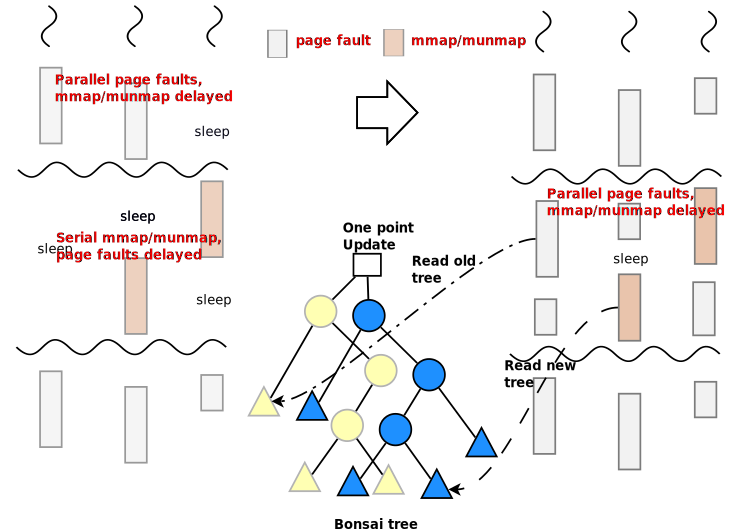
\includegraphics[width=1\textwidth]{fig/bosaivm/bosaivm}
    \caption{Address space 문제와 BosaiVM을 이용한 해결}
  \label{fig:bosaivm}
\end{figure}
 
 
BonsaiVM은 총 3가지 기법을 통해 single address space 문제를 해결하였다. 
%$$$$$$$$$$$$$$$$$$$$$$$$$$$$$$$$$$$$$$$$$$$$$$$$$$$$$$$$$$$$$$$$$$$$$$$$$$$$$$$$
%Paragraph 2: 기법 설명
%$$$$$$$$$$$$$$$$$$$$$$$$$$$$$$$$$$$$$$$$$$$$$$$$$$$$$$$$$$$$$$$$$$$$$$$$$$$$$$$$
Non-blocking synchronization은 장점은 여러 스레드들이 락 기반으로 자원을 관리함에 따라
 발생하는 문제를 해결할 수 있다. 
가장 큰 장점은 스레드 또는 프로세스가 락 때문에 기다리는 시간을 제거할 수 있다.
이 것은 락을 얻기 위해 기다리는 시간을 최소화 할 뿐만 아니라 무한 루프 때문에 무한정 기다리는 
데드락 같은 상황까지 제거 할 수 있다. 
다음으로 모든 락은 락 자체의 오버헤드를 가지고 있는데 이것을 제거할 수 있다. 
예를 들어 코어 수가 증가 할 수록 락 자체를 얻기 위해 원자적 명령을 이용한느데 이것은 캐시 일관성 트래픽을 
발생한다. 
이와 같이 Non-blocking 방법은 이러한 락 자체가 가지고 있는 문제점인 데드락(deadlock), 라이브락(livelock), 
우선순위 역전현상(priority inversion)등을 제거 할 수 있다. 
이러한 Non-blocking synchronization 기법을 사용하는 lock-free 자료 구조들은 성능을 향상 시킬 수 있다. 
그 이유는 멀티코어 환경에서 공유되는 데이터를 접근하기 위해 직렬화 되는 부분이 매우 짧기 때문이다. 


\subsubsection{RadixVM}

%$$$$$$$$$$$$$$$$$$$$$$$$$$$$$$$$$$$$$$$$$$$$$$$$$$$$$$$$$$$$$$$$$$$$$$$$$$$$$$$$
%Paragraph : RadixVM 특징 설명
%$$$$$$$$$$$$$$$$$$$$$$$$$$$$$$$$$$$$$$$$$$$$$$$$$$$$$$$$$$$$$$$$$$$$$$$$$$$$$$$$
RadixVM은 single address space 때문에 발생하는 확장성 문제를 해결하기 위해, 
기존 xv6 운영체제를 대상으로 가상 메모리에 대한 부분을 수정하여 문제를 해결한 연구이다.
그 이유는 리눅스의 가상 메모리를 수정하는 것은 굉잡히 복잡하여,  적용하기 힘들기 떄문에 
덜 복잡한 운영체제에 새로운 개념을 적용하였다. 
RadixVM은 BonsaiVM과 같이 VM의 공유되는 adress space가 map, unmap, page fault 함수 들로 인해 
서로 경쟁함으로 발생하는 문제를 새로운 3가지 접근을 통해 해결하였다. 
첫째로, reference counter와 
--
\begin{figure}[h!]
    \centering
    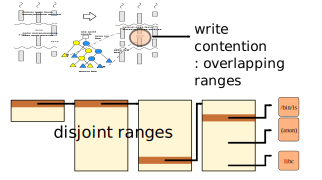
\includegraphics[width=1\textwidth]{fig/radix/radix}
    \caption{RadixVM의 해결 방법}
  \label{fig:radix}
\end{figure}


%$$$$$$$$$$$$$$$$$$$$$$$$$$$$$$$$$$$$$$$$$$$$$$$$$$$$$$$$$$$$$$$$$$$$$$$$$$$$$$$$
%Paragraph : RadixVM  기법 설명 - 1
%$$$$$$$$$$$$$$$$$$$$$$$$$$$$$$$$$$$$$$$$$$$$$$$$$$$$$$$$$$$$$$$$$$$$$$$$$$$$$$$$
Non-blocking synchronization은 장점은 여러 스레드들이 락 기반으로 자원을 관리함에 따라
 발생하는 문제를 해결할 수 있다. 
가장 큰 장점은 스레드 또는 프로세스가 락 때문에 기다리는 시간을 제거할 수 있다.
이 것은 락을 얻기 위해 기다리는 시간을 최소화 할 뿐만 아니라 무한 루프 때문에 무한정 기다리는 
데드락 같은 상황까지 제거 할 수 있다. 
다음으로 모든 락은 락 자체의 오버헤드를 가지고 있는데 이것을 제거할 수 있다. 
예를 들어 코어 수가 증가 할 수록 락 자체를 얻기 위해 원자적 명령을 이용한느데 이것은 캐시 일관성 트래픽을 
발생한다. 
이와 같이 Non-blocking 방법은 이러한 락 자체가 가지고 있는 문제점인 데드락(deadlock), 라이브락(livelock), 
우선순위 역전현상(priority inversion)등을 제거 할 수 있다. 
이러한 Non-blocking synchronization 기법을 사용하는 lock-free 자료 구조들은 성능을 향상 시킬 수 있다. 
그 이유는 멀티코어 환경에서 공유되는 데이터를 접근하기 위해 직렬화 되는 부분이 매우 짧기 때문이다. 


%$$$$$$$$$$$$$$$$$$$$$$$$$$$$$$$$$$$$$$$$$$$$$$$$$$$$$$$$$$$$$$$$$$$$$$$$$$$$$$$$
%Paragraph : RadixVM  기법 설명 - 2
%$$$$$$$$$$$$$$$$$$$$$$$$$$$$$$$$$$$$$$$$$$$$$$$$$$$$$$$$$$$$$$$$$$$$$$$$$$$$$$$
Non-blocking synchronization은 장점은 여러 스레드들이 락 기반으로 자원을 관리함에 따라
 발생하는 문제를 해결할 수 있다. 
가장 큰 장점은 스레드 또는 프로세스가 락 때문에 기다리는 시간을 제거할 수 있다.
이 것은 락을 얻기 위해 기다리는 시간을 최소화 할 뿐만 아니라 무한 루프 때문에 무한정 기다리는 
데드락 같은 상황까지 제거 할 수 있다. 
다음으로 모든 락은 락 자체의 오버헤드를 가지고 있는데 이것을 제거할 수 있다. 
예를 들어 코어 수가 증가 할 수록 락 자체를 얻기 위해 원자적 명령을 이용한느데 이것은 캐시 일관성 트래픽을 
발생한다. 
이와 같이 Non-blocking 방법은 이러한 락 자체가 가지고 있는 문제점인 데드락(deadlock), 라이브락(livelock), 
우선순위 역전현상(priority inversion)등을 제거 할 수 있다. 
이러한 Non-blocking synchronization 기법을 사용하는 lock-free 자료 구조들은 성능을 향상 시킬 수 있다. 
그 이유는 멀티코어 환경에서 공유되는 데이터를 접근하기 위해 직렬화 되는 부분이 매우 짧기 때문이다. 


%Case study of avoiding unintended sharing
 %VM system (ops: map, unmap, page fault)
 %Challenges:
  % reference counters
   %semantics of VM operations
   %when unmap returns page must be unmapped at all cores

%Goal: no intended sharing for VM ops
 % Ops on different memory regions
%  No cache-line transfer when no sharing
 % Ok to have sharing when memory regions overlap
  %  That is intended sharing

%What data structures do we need to maintain?
 % Some information per hardware page (e.g., ppinfo array in jos)
%  Modern OSes don't use an array like jos (too expensive in terms of memory)
 % Modern OSes use a balanced tree
  %  Lock-free balanced trees are tricky
   % Unintended sharing (see figure 6)
    
%Solution: radix tree
 % Behaves like hardware page tables
  %Disjoint lookups/inserts will access disjoint parts of the tree (see figure
  % 7) stores a separate copy of the mapping metadata for each page
  %  metadata also stores pointers to physical memory page
  %Folds repeated entries (unlike jos array)
  %No range queries
  %Freeing nodes in tree using refcache

%TLB shootdown
 % Unmap requires that no core has the page mapped before returning
%  The core running the unmap must send TLB shootdowns to the cores that have
  % the page in their TLB Which cores do have the page in their TLB?
 %   Easy to determine if the processor has a software-filled TLB
  %  At a TLB misses the kernel can record the core # for the page
   % x86 has a hardware-filled TLB
  %Solution: per-core page tables
   % The paging hardware will set the accesses bit only in the per-core page
    % table

%Maps/unmaps for overlapping region
 % simple: locks enforce ordering of concurrent map/unmap on overlapping regions
  %  acquire locks, going left to right
  %page-fault also takes a lock

%Implementation
 % sv6 (C++ version of xv6)
 
 
%Reference counter
  %Design 1: inc, dec+iszero in lock/unlock
   % content on cache-line for lock
  %Design 2: atomic increment/decrement
   % content on cache-line for refcnt
  %Design 3: per-core counters
   % inc/dec: apply op to per-core value
    %iszero: add up all per-core values and check for zero
     % need per-core locks for each counter
    %space overhead is # counters * # cores

%Refcache
 % An object has a shared reference count
%  Per-core cache of deltas
    %inc/dec compute a per-core delta
    %iszero(): applies all deltas to global reference counter
  %If global counter drops to zero, it stays zero
  %Space
   % Uncontended reference counters will be evicted from cache
    %Only cores that use counter have delta

%Challenge: determining if counter is zero
 % Don't want to call iszero() on-demand
  %  it must contact all cores
  %Idea: compute iszero() periodically
   % divide time into epochs (~10 msec)
    %at end of an epoch core flushes deltas to global counter
    %if global counter drops to zero, put on review queue for 2 epochs later
     % if no core has it on its review queue
    %2 epochs later: if global counter is still zero, free object
    %why wait 2 epochs?
  %See example in paper in Figure 1
  %More complications to support weak references

%Epoch maintainance
 % global epoch = min(per-core epochs)
  %each core periodically increase per-core epoch
   % each 10 msec call flush()+review()
  %one core periodically compute global epoch
 

\subsubsection{SC rule}

%$$$$$$$$$$$$$$$$$$$$$$$$$$$$$$$$$$$$$$$$$$$$$$$$$$$$$$$$$$$$$$$$$$$$$$$$$$$$$$$$
%Paragraph : SC rule 특징 및 역사 설명 
%$$$$$$$$$$$$$$$$$$$$$$$$$$$$$$$$$$$$$$$$$$$$$$$$$$$$$$$$$$$$$$$$$$$$$$$$$$$$$$$$
SC rule은 MIT  PDOS 연구 그룹에서 연구한 운영체제의 확장성 개선을 새로운 관점으로 바라본 연구이다. 
기존 연구들은 대부분 운영체제의 병목지점을 추출한 후 이러한 병목지점을 해결하기 위해 새로운 
동기화 기법을 개발하거나 기존 개발된 동기화 기법을 적용하는 방법을 사용하였다. 하지만, 이러한 방법들은 
모두 워크로드가 틀림에 따라 다른 양상을 가지고, 문제를 해결하는데 너무 오랜시간이 걸리는 문제점을 가지고 있다.
실제 확장성에 대한 문제는, 대부분 설계 단계에서 인터페이스를 확장성 있게 소프트웨어를 설계하면 해결된다는 것을 
가지고 새로운 확장성있는 설계에 대해서 초점을 둔 논문이다.
그 이유는 리눅스등의 운영체제는 확장성 있게 설계 되었으나 응용프로그램의 사용방법에 따라 확장성 문제가 발생하기 
때문이다.
파일 시스템을 예를 들어 아래와 같은 명령이 들어오면 확장성이 있으나, 

아래와 같은 명령은 
 
또한, SC rule은 이러한 문제점을 발견하기 위해 메모리의 충돌을 발견하는 새로운 툴을 제안하였다. 
이러한 툴을 통해 설계 단계에서 확장성 문제를 발견할 수 있으며, 이 툴을 통해 기존 운영체제(리눅스, sv6)를 
분석하였다. 

%$$$$$$$$$$$$$$$$$$$$$$$$$$$$$$$$$$$$$$$$$$$$$$$$$$$$$$$$$$$$$$$$$$$$$$$$$$$$$$$$
%Paragraph : SC rule 예제 설명 
%$$$$$$$$$$$$$$$$$$$$$$$$$$$$$$$$$$$$$$$$$$$$$$$$$$$$$$$$$$$$$$$$$$$$$$$$$$$$$$$$
Non-blocking synchronization은 장점은 여러 스레드들이 락 기반으로 자원을 관리함에 따라
 발생하는 문제를 해결할 수 있다. 
가장 큰 장점은 스레드 또는 프로세스가 락 때문에 기다리는 시간을 제거할 수 있다.
이 것은 락을 얻기 위해 기다리는 시간을 최소화 할 뿐만 아니라 무한 루프 때문에 무한정 기다리는 
데드락 같은 상황까지 제거 할 수 있다. 
다음으로 모든 락은 락 자체의 오버헤드를 가지고 있는데 이것을 제거할 수 있다. 
예를 들어 코어 수가 증가 할 수록 락 자체를 얻기 위해 원자적 명령을 이용한느데 이것은 캐시 일관성 트래픽을 
발생한다. 
이와 같이 Non-blocking 방법은 이러한 락 자체가 가지고 있는 문제점인 데드락(deadlock), 라이브락(livelock), 
우선순위 역전현상(priority inversion)등을 제거 할 수 있다. 
이러한 Non-blocking synchronization 기법을 사용하는 lock-free 자료 구조들은 성능을 향상 시킬 수 있다. 
그 이유는 멀티코어 환경에서 공유되는 데이터를 접근하기 위해 직렬화 되는 부분이 매우 짧기 때문이다. 


%\subsubsection{FS scalability}



%BonsaiVM~\cite{AustinTClements2012RCUBalancedTrees} solved this address space
%problem by using the RCU;
%RadixVM~\cite{Clements2013RadixVM} created a new VM using refcache and radix
%tree, which enable \code{munmap}, \code{mmap}, and \code{page fault} on
%non-overlapping memory regions to scale perfectly.
%Alternatively, to avoid contention caused by shared address space locking,
%system programmers change their multithreaded applications to use
%processes~\cite{SilasBoydWickizer2010LinuxScales48}.

